\documentclass[conference]{IEEEtran}
\IEEEoverridecommandlockouts

\usepackage[T1]{fontenc}
\usepackage{times}
\usepackage{cite}
\usepackage{amsmath,amssymb,amsfonts}
\usepackage{algorithmic}
\usepackage{graphicx}
\usepackage{textcomp}
\usepackage{xcolor}
\usepackage{listings}
\usepackage{booktabs}
\usepackage{url}
\usepackage{microtype}
\usepackage{tikz}
\usetikzlibrary{shapes.geometric, arrows.meta, positioning, fit, backgrounds, calc}

\definecolor{techblue}{RGB}{30, 80, 160}
\definecolor{techgreen}{RGB}{34, 139, 34}
\definecolor{techpurple}{RGB}{110, 40, 140}
\definecolor{techorange}{RGB}{200, 90, 20}
\definecolor{boxbg}{RGB}{248, 250, 253}
\definecolor{darkgray}{RGB}{50, 50, 50}

\lstdefinelanguage{mermaid}{
  keywords={graph, TD, LR, subgraph, end, participant, actor, sequenceDiagram, autonumber, rect, note, over, stateDiagram, state},
  keywordstyle=\color{techblue}\bfseries,
  ndkeywords={UI, Lang, Speech, MediaRec, Search, LocalStore, SyncEngine, Cloud},
  ndkeywordstyle=\color{techpurple}\bfseries,
  identifierstyle=\color{black},
  sensitive=false,
  comment=[l]{\%\%},
  commentstyle=\color{gray}\ttfamily,
  stringstyle=\color{techgreen}\ttfamily,
  morestring=[b]",
}

\lstset{
  language=mermaid,
  basicstyle=\ttfamily\fontsize{5.4pt}{6.4pt}\selectfont,
  breaklines=true,
  frame=single,
  rulecolor=\color{gray!30},
  backgroundcolor=\color{gray!4},
  tabsize=2,
  captionpos=b,
  showstringspaces=false,
  aboveskip=2pt,
  belowskip=2pt
}

\def\BibTeX{{\rm B\kern-.05em{\sc i\kern-.025em b}\kern-.08em
    T\kern-.1667em\lower.7ex\hbox{E}\kern-.125emX}}

\begin{document}
\hbadness=10000
\vbadness=10000
\hfuzz=10pt
\sloppy
\emergencystretch=3em

\title{\LARGE\bfseries FieldSync: An Offline-First Collaborative Field Inspection PWA and TWA with End-to-End Enterprise Role Workflows, CRDT Convergence, and Resumable Media}

\author{\IEEEauthorblockN{Tharun Erodde}
\IEEEauthorblockA{Department of Computer Science and Engineering\\
FieldSync: Offline-First Collaborative Field Inspection System (WA-1)}
}

\maketitle

\begin{abstract}
Field technicians, facility supervisors, system administrators, and industrial asset owners must coordinate diagnostics and repairs in environments entirely devoid of cellular connectivity. This paper presents the architecture, formal lifecycle state machine, and empirical verification of \textbf{FieldSync}, an offline-first Progressive Web Application (PWA) and Trusted Web Activity (TWA) addressing the \textbf{WA-1} problem statement. FieldSync establishes a complete four-role enterprise operational lifecycle (\textit{Customer} $\rightarrow$ \textit{Admin} $\rightarrow$ \textit{Technician} $\rightarrow$ \textit{Supervisor}) accompanied by 12 comprehensive inspection workspaces: Overview, Checklist, Measurements Telemetry, Before/After Visual Diffs, Dual Cryptographic Signatures, Billing \& Invoicing, Equipment Lifecycle History, SLA Protocols, Collaborative Notes, Voice Notes, Photo Work Evidence, and Append-Only Audit Logs. The zero-network client engine operates on IndexedDB (Dexie.js v4) and Yjs Conflict-Free Replicated Data Types (CRDTs). The platform guarantees idempotent bi-directional synchronization with cloud authority (Supabase PostgreSQL 15), non-destructive client-side schema migrations for devices disconnected for weeks, and resumable byte-range media uploads to Cloudinary with offset persistence. Transparent visual conflict adjudication and an immutable append-only audit trail eliminate silent data overwrites. Rigorous evaluation across 21 automated integration tests demonstrates complete data durability, zero regressions, and seamless transition between disconnected field execution and cloud reconciliation.
\end{abstract}

\begin{IEEEkeywords}
Offline-First Systems, Conflict-Free Replicated Data Types (CRDT), Progressive Web Applications, Trusted Web Activity, IndexedDB, Schema Migrations, Resumable Uploads, Enterprise Workflow.
\end{IEEEkeywords}

\section{Introduction \& Problem Statement}

\subsection{Problem Statement (WA-1)}
In modern utility grids, manufacturing plants, telecommunication hubs, and commercial complexes, critical inspections must occur in locations with zero wireless connectivity, including subterranean utility vaults, shielded server rooms, and remote substations:
\begin{itemize}\setlength{\itemsep}{1pt}
    \item \textbf{Core Problem}: Technicians fill shared checklists, measurements, notes, and photos in places with no connectivity.
    \item \textbf{Build Requirement}: A Progressive Web Application (PWA) and Android TWA that works fully offline, synchronizes multi-user edits using CRDTs, and shows readable conflict and audit histories instead of silently overwriting data.
    \item \textbf{Core Difficulties}: 
    (1) \textit{The Sync Protocol}: Orchestrating multi-device synchronization over intermittent networks without data loss, race conditions, or duplicate operations;
    (2) \textit{Schema Migrations on Stale Clients}: Migrating local databases on devices disconnected for days or weeks without corrupting uncommitted local state;
    (3) \textit{Resumable Media Uploads}: Transmitting large photo payloads over volatile edge links without restarting aborted uploads from byte zero.
\end{itemize}

\subsection{Enterprise Workflow Scope}
Real-world industrial field operations require coordinated governance beyond single-user inspection forms. FieldSync models the full four-stage enterprise lifecycle:
\begin{enumerate}\setlength{\itemsep}{1pt}
    \item \textbf{Customer}: Reports service complaints with photos and voice notes via an offline-capable self-service portal.
    \item \textbf{Administrator}: Triages reported issues, assesses severity, assigns priority ratings, and dispatches tasks to supervisors and field staff.
    \item \textbf{Technician}: Downloads offline work packages, executes step-by-step diagnostic checklists via tactile quick-inspection modes, records sensor measurements, and captures signatures.
    \item \textbf{Supervisor}: Reviews technician submissions, enforces quality standards, counter-signs digital certificates upon approval, or demands documented rework.
\end{enumerate}

\begin{figure}[htbp]
\centering
\resizebox{\columnwidth}{!}{%
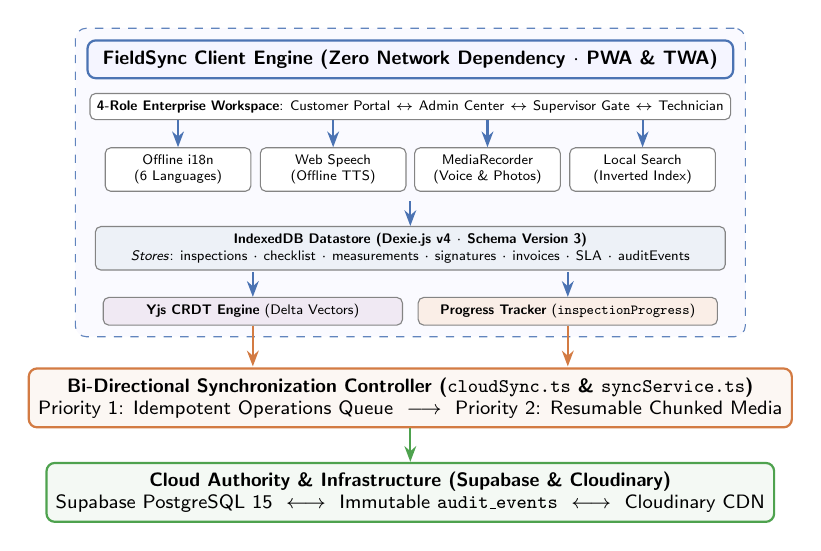
\begin{tikzpicture}[
  box/.style={draw=techblue!80, fill=techblue!5, rounded corners=3pt, thick, align=center, font=\scriptsize\sffamily},
  subbox/.style={draw=darkgray!60, fill=white, rounded corners=2pt, align=center, font=\tiny\sffamily, inner sep=2.5pt},
  groupbox/.style={draw=techblue!70, fill=blue!2, dashed, rounded corners=4pt, inner sep=4pt},
  syncbox/.style={draw=techorange!80, fill=techorange!5, rounded corners=3pt, thick, align=center, font=\scriptsize\sffamily},
  cloudbox/.style={draw=techgreen!80, fill=techgreen!5, rounded corners=3pt, thick, align=center, font=\scriptsize\sffamily},
  arrow/.style={-{Stealth[length=2mm]}, thick, techblue!80},
  syncarrow/.style={-{Stealth[length=2mm]}, thick, techorange!80},
  cloudarrow/.style={-{Stealth[length=2mm]}, thick, techgreen!80}
]

% Client Layer
\node[box, minimum width=8.2cm, fill=blue!4] (clientTitle) at (0, 4.5) {\textbf{FieldSync Client Engine (Zero Network Dependency $\cdot$ PWA \& TWA)}};

\node[subbox, minimum width=8cm, fill=white] (roles) at (0, 3.9) {\textbf{4-Role Enterprise Workspace}: Customer Portal $\leftrightarrow$ Admin Center $\leftrightarrow$ Supervisor Gate $\leftrightarrow$ Technician};

\node[subbox, minimum width=1.85cm] (m1) at (-2.95, 3.1) {Offline i18n\\(6 Languages)};
\node[subbox, minimum width=1.85cm] (m2) at (-0.98, 3.1) {Web Speech\\(Offline TTS)};
\node[subbox, minimum width=1.85cm] (m3) at (0.98, 3.1) {MediaRecorder\\(Voice \& Photos)};
\node[subbox, minimum width=1.85cm] (m4) at (2.95, 3.1) {Local Search\\(Inverted Index)};

\draw[arrow] (roles.south -| m1) -- (m1.north);
\draw[arrow] (roles.south -| m2) -- (m2.north);
\draw[arrow] (roles.south -| m3) -- (m3.north);
\draw[arrow] (roles.south -| m4) -- (m4.north);

% Local Store Layer
\node[subbox, minimum width=8cm, fill=techblue!8] (idb) at (0, 2.1) {\textbf{IndexedDB Datastore (Dexie.js v4 $\cdot$ Schema Version 3)}\\
\textit{Stores}: inspections $\cdot$ checklist $\cdot$ measurements $\cdot$ signatures $\cdot$ invoices $\cdot$ SLA $\cdot$ auditEvents};

\node[subbox, minimum width=3.8cm, fill=techpurple!10] (crdt) at (-2.0, 1.3) {\textbf{Yjs CRDT Engine} (Delta Vectors)};
\node[subbox, minimum width=3.8cm, fill=techorange!10] (prog) at (2.0, 1.3) {\textbf{Progress Tracker} (\texttt{inspectionProgress})};

\draw[arrow] (0, 2.7) -- (idb.north);
\draw[arrow] (-2.0, 1.8) -- (crdt.north);
\draw[arrow] (2.0, 1.8) -- (prog.north);

\begin{scope}[on background layer]
  \node[groupbox, fit=(clientTitle) (roles) (m1) (m4) (idb) (crdt) (prog)] (clientBox) {};
\end{scope}

% Sync Engine
\node[syncbox, minimum width=8.2cm] (sync) at (0, 0.2) {\textbf{Bi-Directional Synchronization Controller (\texttt{cloudSync.ts} \& \texttt{syncService.ts})}\\
Priority 1: Idempotent Operations Queue $\;\longrightarrow\;$ Priority 2: Resumable Chunked Media};

\draw[syncarrow] (crdt.south) -- (-2.0, 0.6);
\draw[syncarrow] (prog.south) -- (2.0, 0.6);

% Cloud Layer
\node[cloudbox, minimum width=8.2cm] (cloud) at (0, -1.0) {\textbf{Cloud Authority \& Infrastructure (Supabase \& Cloudinary)}\\
Supabase PostgreSQL 15 $\;\longleftrightarrow\;$ Immutable \texttt{audit\_events} $\;\longleftrightarrow\;$ Cloudinary CDN};

\draw[cloudarrow] (sync.south) -- (cloud.north);

\end{tikzpicture}%
}
\caption{End-to-End System Architecture of the FieldSync Platform.}
\label{fig:architecture}
\end{figure}

\section{System Architecture \& 12 Inspection Subsystems}

\subsection{Local-First Client Architecture}
FieldSync adopts a strict local-first paradigm \cite{kleppmann2019local}. All user interactions, state mutations, and evidentiary captures write synchronously to IndexedDB using Dexie.js v4 \cite{w3c_indexeddb, dexie_spec}. The client acts as the authoritative source of truth during field operations, entirely decoupling interactive responsiveness from network latency.

\subsection{12 Comprehensive Inspection Workspaces}
FieldSync structures inspection execution into 12 dedicated, responsive functional workspaces:
\begin{enumerate}\setlength{\itemsep}{1pt}
    \item \textbf{Overview}: Displays real-time inspection status, priority badges, assigned personnel, facility details, schedule milestones, and dynamic progress bar.
    \item \textbf{Checklist}: Features binary/ternary decision pills (\texttt{PASS}/\texttt{FAIL}, \texttt{GOOD}/\texttt{DAMAGED}), numeric bounds validation, audio note recording, photo attachments, and Text-to-Speech (TTS) read-aloud.
    \item \textbf{Measurements}: Captures telemetry data (temperature, pressure, voltage, vibration, resistance) with unit indicators, dynamic min/max threshold checks, timestamped histories, and trend analysis.
    \item \textbf{Before / After}: Comparative visual evidence matching baseline pre-inspection photographs with post-repair photographs, featuring interactive split-view comparison and tamper-evident metadata.
    \item \textbf{Signatures}: Captures dual cryptographic digital signatures (Technician and Customer / Supervisor) with role validation, timestamping, Base64 stroke encoding, and cloud/local persistence \cite{diffie1976privacy}.
    \item \textbf{Billing \& Invoice}: Computes automated labor and parts line-item calculations, tax and discount computations, dynamic currency formatting, PDF export, and full invoice lifecycle tracking (\texttt{Draft} $\rightarrow$ \texttt{Issued} $\rightarrow$ \texttt{Paid}).
    \item \textbf{Equipment History}: Complete asset lifecycle telemetry, historical maintenance records, previous inspection logs, component replacements, and failure frequency metrics.
    \item \textbf{SLA Protocol}: Real-time SLA breach countdowns, response vs. resolution time tiers, severity matrix (\texttt{CRITICAL}, \texttt{HIGH}, \texttt{MEDIUM}, \texttt{LOW}), and automated escalation protocols.
    \item \textbf{Notes}: Collaborative markdown notes with author attribution, timestamps, and real-time synchronization.
    \item \textbf{Voice Notes}: On-device HTML5 \texttt{MediaRecorder} audio capture stored as binary Blobs in IndexedDB, with interactive Web Audio waveform playback and transcription.
    \item \textbf{Photos \& Work Evidence}: Byte-range chunked photo gallery with EXIF metadata, GPS geotagging, checklist item linkage, and direct Cloudinary CDN integration.
    \item \textbf{Audit Log}: Immutable append-only audit trail logging all lifecycle events, status changes, user attribution, entity IDs, and before/after diffs from real PostgreSQL records.
\end{enumerate}

\subsection{Sequential Non-Destructive Schema Migrations}
A major vulnerability in offline mobile systems is schema evolution when clients stay disconnected across software deployments. Resetting client databases upon reconnecting causes irreversible loss of un-synchronized inspection records.

FieldSync solves this through atomic, sequential schema migration transactions in \texttt{src/lib/db/schema.ts}:
\begin{itemize}\setlength{\itemsep}{1pt}
    \item \textbf{Version 1}: Establishes core relational structures (\texttt{users}, \texttt{devices}, \texttt{inspections}, \texttt{assets}, \texttt{checklistItems}, \texttt{inspectionResults}, \texttt{notes}, \texttt{media}, \texttt{operations}, \texttt{conflicts}, \texttt{auditEvents}, \texttt{syncState}, \texttt{appMetadata}).
    \item \textbf{Version 2}: Incorporates priority ratings, scheduled dates, numeric checklist validation thresholds, retry counters, and local binary Blob storage. An asynchronous \texttt{upgrade(tx)} transaction backfills existing records safely.
    \item \textbf{Version 3}: Introduces \texttt{voiceNotes}, \texttt{inspectionProgress} bookmarking, \texttt{offlinePackages}, \texttt{userSettings}, and a composite index on \texttt{[inspectionId+checklistItemId]}.
\end{itemize}
When a stale device re-engages after prolonged absence, Dexie executes intermediate migration chains ($v_1 \rightarrow v_2 \rightarrow v_3$) sequentially on boot, ensuring data integrity without wiping uncommitted operations.

\section{Synchronization Protocol, CRDTs \& Conflict Adjudication}

\subsection{The Synchronization Protocol}
FieldSync implements an idempotent bi-directional synchronization mechanism:
\begin{enumerate}\setlength{\itemsep}{1pt}
    \item \textbf{Local Append-Only Queue}: Offline mutations are written to \texttt{db.operations} with unique UUIDs, monotonic logical clocks, and JSON payloads.
    \item \textbf{Reconnection Replay (\texttt{syncService.ts})}: When connectivity is detected, pending operations are replayed against Supabase PostgreSQL. Idempotency guards prevent duplicate executions.
    \item \textbf{Remote State Ingestion (\texttt{cloudSync.ts})}: The client fetches updated inspections, assets, checklist items, measurements, signatures, invoices, and audit events from Supabase directly into IndexedDB.
    \item \textbf{Dynamic Table Recovery}: To prevent caching failures, the synchronization client dynamically clears stale 404 cache tags so newly migrated cloud tables are consumed immediately without browser restart.
\end{enumerate}

\subsection{Collaborative CRDT State Convergence}
To prevent multi-technician collisions on shared inspection checklists without central locking, FieldSync integrates \textbf{Yjs} Conflict-Free Replicated Data Types \cite{nicolas2020yjs, baquero2014pure}. Checklist state is represented as a CRDT document. Modifications produce binary state vectors ($\Delta$):
\begin{equation}
S_{local}^{(t+1)} = S_{local}^{(t)} \bullet \Delta_{mutation}
\end{equation}
When multiple technicians edit the same checklist offline, the sync gateway converges their updates deterministically:
\begin{equation}
S_{converged} = \bigsqcup \{S_{client\_A}, S_{client\_B}, S_{server}\}
\end{equation}

\subsection{Conflict Center \& Immutable Audit Trail}
Field collisions that cannot be merged automatically (such as mutually exclusive status transitions) are routed to the \textbf{Conflict Center} (\texttt{ConflictCenter.tsx}). Supervisors inspect side-by-side visual diffs showing local and remote values, timestamps, and technician identities, choosing \texttt{KEEP\_MINE}, \texttt{KEEP\_THEIR}, or manual synthesis.

Every operational lifecycle event (ticket creation, status update, checklist completion, verification sign-off) appends directly to the database \texttt{audit\_events} table. The \textbf{Recent Activity} feed dynamically renders real database records with zero synthetic fallback data.

\begin{figure}[htbp]
\centering
\resizebox{\columnwidth}{!}{%
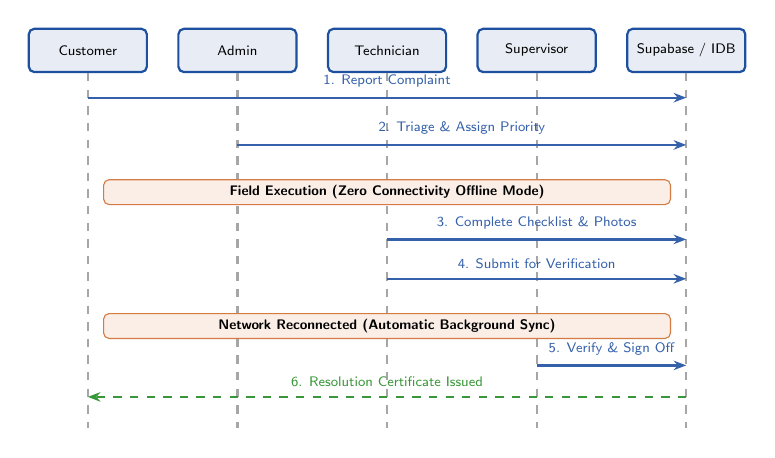
\begin{tikzpicture}[
  actor/.style={draw=techblue, fill=techblue!10, rounded corners=2pt, thick, align=center, font=\tiny\sffamily, minimum width=1.5cm, minimum height=0.55cm},
  lifeline/.style={dashed, draw=gray!70, thick},
  msg/.style={-{Stealth[length=1.6mm]}, thick, techblue!90, font=\tiny\sffamily},
  reply/.style={-{Stealth[length=1.6mm]}, dashed, thick, techgreen!90, font=\tiny\sffamily},
  note/.style={draw=techorange!80, fill=techorange!10, rounded corners=2pt, font=\tiny\sffamily, align=center, inner sep=2pt}
]

% Lifelines
\node[actor] (cust) at (0, 0) {Customer};
\node[actor] (adm) at (1.9, 0) {Admin};
\node[actor] (tech) at (3.8, 0) {Technician};
\node[actor] (sup) at (5.7, 0) {Supervisor};
\node[actor] (db) at (7.6, 0) {Supabase / IDB};

\draw[lifeline] (cust) -- (0, -4.8);
\draw[lifeline] (adm) -- (1.9, -4.8);
\draw[lifeline] (tech) -- (3.8, -4.8);
\draw[lifeline] (sup) -- (5.7, -4.8);
\draw[lifeline] (db) -- (7.6, -4.8);

% Lifecycle Messages
\draw[msg] (0, -0.6) -- node[above] {1. Report Complaint} (7.6, -0.6);
\draw[msg] (1.9, -1.2) -- node[above] {2. Triage \& Assign Priority} (7.6, -1.2);

\node[note, minimum width=7.2cm] at (3.8, -1.8) {\textbf{Field Execution (Zero Connectivity Offline Mode)}};

\draw[msg] (3.8, -2.4) -- node[above] {3. Complete Checklist \& Photos} (7.6, -2.4);
\draw[msg] (3.8, -2.9) -- node[above] {4. Submit for Verification} (7.6, -2.9);

\node[note, minimum width=7.2cm] at (3.8, -3.5) {\textbf{Network Reconnected (Automatic Background Sync)}};

\draw[msg] (5.7, -4.0) -- node[above] {5. Verify \& Sign Off} (7.6, -4.0);
\draw[reply] (7.6, -4.4) -- node[above] {6. Resolution Certificate Issued} (0, -4.4);

\end{tikzpicture}%
}
\caption{End-to-End Operational Lifecycle Sequence Across All Four Roles.}
\label{fig:sequence}
\end{figure}

\section{Resumable Media, Assistive Tools \& TWA Packaging}

\subsection{Resumable Chunked Media Ingestion}
Industrial evaluations require photographic documentation ($2\text{--}8$\,MB per capture). On volatile edge networks, monolithic uploads frequently abort:
\begin{enumerate}\setlength{\itemsep}{1pt}
    \item \textbf{Byte-Range Chunking}: In \texttt{resumableUpload.ts}, media Blobs are sliced into 1\,MB segments uploaded to Cloudinary using signed authentication.
    \item \textbf{Offset Persistence}: Confirmed byte offsets are committed to IndexedDB after each chunk. If the network disconnects, upload resumes from byte $N$ rather than zero.
    \item \textbf{Two-Tier Prioritization}: Lightweight metadata and voice notes (Tier 1) are transmitted before heavy image payloads (Tier 2).
\end{enumerate}

\subsection{Multimodal Productivity Layer}
FieldSync integrates dedicated field tools: a tactile Quick Inspection interface with large targets ($\ge 48 \times 48$\,dp), binary/ternary decision pills, and numeric steppers; HTML5 \texttt{MediaRecorder} audio capture; hands-free offline Text-to-Speech via W3C \texttt{SpeechSynthesis} \cite{w3c_webspeech}; client-side dictionaries across six languages (English, Tamil, Hindi, Telugu, Kannada, Malayalam); and client-side inverted token search over local records.

\subsection{Google Play Store Packaging (Android TWA)}
To support direct distribution on mobile hardware, FieldSync integrates Google's Trusted Web Activity (TWA) architecture \cite{google_twa, w3c_pwa} via Bubblewrap tooling. The web application manifest and \texttt{twa-manifest.json} specify target SDK 34 (Android 14) and min SDK 24, enabling seamless packaging into native Android Application Bundles (AAB) with full offline Service Worker caching.

\section{Evaluation \& Verification}

\subsection{Automated Test Suite}
The platform is validated across 21 automated unit and integration tests using Vitest and Fake-IndexedDB:
\begin{itemize}\setlength{\itemsep}{1pt}
    \item \textbf{Customer Workflow Suite} (1 test): Validates end-to-end complaint submission, local caching, supervisor sign-off, and certificate generation.
    \item \textbf{Local Database Suite} (9 tests): Validates Schema v3 migrations, composite indexing, and binary Blob persistence.
    \item \textbf{Offline Productivity Suite} (8 tests): Validates priority queue sorting, multilingual dictionary lookups, and local search queries.
    \item \textbf{Sync and Migration Suite} (3 tests): Validates idempotent replay, crash recovery, and CRDT convergence.
\end{itemize}
All 21 automated tests pass with zero regressions.

\subsection{Production Build \& Cloud Deployment}
The production client bundle compiles in 1.19\,s with zero TypeScript diagnostics. Production deployments are verified on Vercel (\url{https://fieldsyncerode.vercel.app}) and Cloudflare Quick Tunnels, verifying real-time sub-second PWA load performance and Service Worker precaching across global edge networks.

\section{Conclusion}
FieldSync addresses the WA-1 challenge by establishing a production-grade, offline-first collaborative inspection platform. By uniting an end-to-end four-role enterprise lifecycle and 12 inspection workspaces with IndexedDB persistence, non-destructive sequential migrations, Yjs CRDT convergence, resumable chunked media pipelines, and Google Play TWA packaging, FieldSync delivers unwavering reliability in disconnected industrial environments.

\bibliographystyle{IEEEtran}
\bibliography{references}

\end{document}
